\documentclass[a4paper,12pt,oneside]{article}
% Palatino font
\usepackage{graphicx,apalike,hyperref,rotating,longtable,pslatex,sectsty}
\sectionfont{\fontsize{12}{15}\selectfont}
\subsectionfont{\fontsize{12}{15}\selectfont}
\renewcommand{\baselinestretch}{1.5}
\usepackage[nottoc,notlot,notlof]{tocbibind}
\usepackage[
    top    = 2.00cm,
    bottom = 2.00cm,
    left   = 2.50cm,
    right  = 2.50cm]{geometry}
\hypersetup{
    colorlinks,%
    citecolor=black,%
    filecolor=black,%
    linkcolor=black,%
    urlcolor=black,%
    pdfmenubar=true
}
% Change line spacing for figure captions
\usepackage{caption,setspace}
\captionsetup[figure]{labelfont=bf,labelsep=period}

\author{Yuvia Alhel\'i P\'erez Rico}
\begin{document}

	\begin{titlepage}
		\begin{minipage}{0.25\textwidth}
			\begin{flushleft}
				
\includegraphics[width=4cm,height=3cm]{./figures/ens1.jpg}
			\end{flushleft}
		\end{minipage}
		\begin{minipage}{0.75\textwidth}
			\begin{center}		
				\'ECOLE NORMALE SUP\'ERIEURE
				\rule{11.5cm}{0.25mm}\vspace{-4.5mm}
				\rule{11.5cm}{1.5mm}\\[1.5mm]
				INTERDISCIPLINARY MASTER IN LIFE SCIENCES\\\vspace{0.7mm}IMaLiS year 2
			\end{center}
		\end{minipage}
		\begin{minipage}{0.25\textwidth}
			\vspace{0.4cm}
			\begin{center}
				\rule{0.25mm}{0.85\textheight}\hspace{0.5mm}
				\rule{1.5mm}{0.85\textheight}\hspace{0.5mm}
				\rule{0.25mm}{0.85\textheight}
			\end{center}
		\end{minipage}	
		\begin{minipage}{0.85\textwidth}
			\begin{center}
				\vspace{3.5cm}
				\textbf{Comparative Analysis of Enhancers and Super-Enhancers\\Reveals Conserved Elements in Vertebrate Genomes}\\[1cm]
				by\\[0.5cm]YUVIA ALHEL\'I P\'EREZ RICO\\[3.5cm]
				A REPORT SUBMITTED\\\vspace{0.7mm}IN PARTIAL FULFILLMENT\\\vspace{0.7mm}OF THE REQUIREMENTS FOR THE DEGREE OF\\\vspace{0.7mm}\emph{MASTER IN LIFE SCIENCES}\\[3cm]
				SUPERVISOR: ALENA SHKUMATAVA\\\vspace{0.7mm}LONG INTERVENING NONCODING RNAs\\IN VERTEBRATE DEVELOPMENT\\INSTITUT CURIE\\[0.3cm]
				\begin{center}
					\begin{tabular}{l r}
						PARIS, FRANCE\hspace{2cm} & JUNE 2014
					\end{tabular}
				\end{center}
			\end{center}
		\end{minipage}

	\end{titlepage}

	\newpage

	\begin{center}
		\textbf{Abstract}
	\end{center}
		Genome-wide analyses of \textit{cis}-regulatory elements have highlighted the relevance of these elements in global transcriptional regulation. Among these \textit{cis}-elements enhancers have arisen as key regulators of gene expression. Recent publications have reported the presence of stretch enhancers in privileged regions of hyperactive chromatin in mammalian cells and tissues. Clusters of stretch enhancers, referred as super-enhancers, are characterized by a high abundance of master transcription factors, transcriptional coactivators and chromatin remodelers. Strikingly, super-enhancer targets include genes important for the establishment of cell identity, suggesting that super-enhancers could operate at the nexus of transcriptional networks that define cell states. Despite their important regulatory function, it is not known if super-enhancers exist outside of mammals. In this study, we generated enhancer maps for zebrafish and identified for the first time super-enhancers in a non-mammalian organism. In addition, we identified new enhancers and super-enhancers in mouse and human cells as well as adult tissue. Our cross-species comparison showed that zebrafish super-enhancers share key features with mammalian super-enhancers such as extension and association with identity genes. Moreover, we found that a considerable number of  enhancers and super-enhancers are conserved across distant vertebrate genomes. The enhancer roadmaps generated here set the stage for future functional and structural enhancer studies, particularly those focusing on non-mammalian vertebrates.\\

	\newpage

	\tableofcontents

	\newpage

	\section{Introduction}

	Gene expression is controlled by a series of transcriptional and post-transcriptional events that culminate in spatio/temporal expression of genes relevant to a particular cell state. Transcriptional regulation depends on promoters and \textit{cis}-regulatory elements that facilitate the assembly of the transcriptional machinery at transcription start sites (TSSs) (Darnell, 2011). It is well known that promoters are sufficient to recruit RNA polymerase to TSSs. However, in these conditions transcription either cannot be initiated or it is maintained at low rates, and can only be triggered or enhanced by the action of \textit{cis}-regulatory elements (Adelman and Lis, 2012).\\

	Among \textit{cis}-regulators, enhancers have primordial roles in the orchestration of transcriptional networks (Smith and Shilatifard, 2014). Enhancers are DNA sequences that recruit transcription factors and transcriptional coactivators to TSSs to stimulate transcription of their target genes. Moreover, enhancers are able to function over long genomic distances from their target genes and their functions are independent of sequence context. Therefore, there is no correlation between promoter and enhancer orientations (Darnell, 2011). The identification of enhancers based on their properties and functions (reviewed in Shlyueva et al., 2014) has begun to shed light on the complexity of transcriptional regulation. And now, it is becoming increasingly evident that enhancer landscapes change according to cell type, and that these changes are involved in complex processes such as development (Kieffer-Kwon et al., 2013; Nord et al., 2013).\\

	Previously, the enrichment of RNA polymerase II and general transcription factors at putative enhancers in mouse T cells allowed the identification of transcription initiation platforms (Koch et al., 2011). These platforms showed preferential association with tissue-specific genes, and the observed specificity increased with the size of the platform. More recently, Whyte et al. (2013) and Lov\'en et al. (2013) reported the existence of hyperactive chromatin clusters of stretch enhancers characterized by high density levels of transcriptional coactivators and transcription factors controlling cell fate. As in the case of transcription initiation platforms, stretch enhancers or super-enhancers are preferentially associated with tissue-specific genes and in particular with key identity genes. It was also reported that super-enhancers can induce higher levels of transcription of their target genes than regular enhancers. In addition, super-enhancer functions are more sensitive to perturbations at the levels of their binding factors. Altogether, these observations suggest that super-enhancers are main players in the establishment of cell states in homeostasis and disease (Lov\'en et al., 2013; Parker et al., 2013; Hnisz et al., 2013).\\ 

	New studies in adipocite cells have revealed that most super-enhancers contain sequence modules that correspond to transcription factor hotspots (Siersb\ae k, 2014), where different transcription factors can bind cooperatively to regulate transcription of their target genes. Given that various combinations of transcription factors are observed at hotspots it is unlikely that their binding to those regions is a consequence of random associations with open chromatin (Siersb\ae k, 2011; Siersb\ae k, 2014). Rather, it is likely that the combinatorial arrangement of transcription factors is dictated by specific signals. Although the arrangement of transcription factor profiles of hotspots is just starting to be understood (Siersb\ae k, 2014), it is provoking to think that super-enhancer functions may reside in these types of modules.\\

	Considering their relation with transcriptional regulation and with target genes often misregulated in disease states, super-enhancers appear as possible therapeutic targets (Lov\'en et al., 2013). However, the existence of stretch enhancers has only been reported in mammalian cells and tissues, restricting their analysis to a few model organisms. Consequently, it is important to determine if super-enhancers are also present in non-mammalian model organisms, such as zebrafish, which is increasingly becoming a model organism for the study of human genetic diseases (Howe et al., 2013; Vacaru et al, 2014). Furthermore, it is also important to determine if these elements are conserved across vertebrates. In this study, we begin to respond to these unknown factors by first establishing genome-wide enhancer maps and then analyzing and comparing these maps to those of mouse and human. Consistent with their presence in active chromatin, active enhancers are labelled by the acetylation of histone H3 at the lysine 27 residue (H3K27ac) (Creyghton et al., 2010). Noteworthy, this histone modification has been reported to better recapitulate the identification of super-enhancers based on master transcription factors and Mediator (Hnisz et al., 2013). For this reason, we decided to analyze the H3K27ac profiles of different cells and tissues to assess the relationship between vertebrate enhancers and super-enhancers.\\



	\section{Materials and Methods}

	\subsection{Chomatin immunoprecipitation sequencing (ChIP-seq)}

		Whole brains were dissected from adult zebrafish of mixed gender and separated in two biological replicates. For the chromatin immunoprecipitation assays around \(2.5x10^{8}\) cells were used per replicate. Cells were crosslinked with 1\% formaldehyde for 15 minutes and subsequently formaldehyde was quenched with glycine (0.125 $M$). Chromatin was sonicated and immunoprecipitated with 100 \(\mu l\) of antibody/magnetic bead mix. To prepare this mix 6 \(\mu g\) of H3K27ac antibody (Abcam, ab4729) were incubated with magnetic beads over night at $4\,^{\circ}\mathrm{C}$. For each ChIP assay 50 \(\mu l\) of sonicated chromatin was kept as input DNA. The immunoprecipitated chromatin and inputs were reverse-crosslinked. All samples were treated with RNase A and proteinase K and resuspended in 30 \(\mu l\) of 10 $mM$ Tris-HCl pH 8. DNA fragments with an average size of 350 bp were used for single-end library preparation following Illumina protocols. All libraries were sequenced twice in a HiSeq 2500 machine.\\

	\subsection{Analysis of ChIP-seq data sets}

		Libraries were mapped with \texttt{Bowtie 2} (Langmead and Salzberg, 2012) to their corresponding reference genome (danRer7 for zebrafish, mm10 for mouse and hg38 for human) allowing up to 1 mismatch in the seed and saving alignments as SAM files. SAM files were converted to BAM files with \texttt{samtools} (Li et al., 2009). Given that no peak caller able to handle biological replicates has been published, BAM files from technical and biological replicates were merged. BAM files were filtered to discard alignments with mapping quality $<20$ and converted to BED files using \texttt{BEDTools} (Quinian and Hall, 2010). Peak calling was performed with \texttt{SICER} (Zang et al., 2009) setting window size to 200, redundancy threshold to 1, gap size to 600, false discovery rate to 0.05 and changing the fragment size accordingly to the data set analyzed. All data sets were analyzed using input libraries as control, except the dome-stage data set for zebrafish, for which no input library was available. WIG files for ChIP-seq libraries were created with \texttt{FindPeaks} (Fejes et al., 2008) using the \textsl{-duplicatefilter} option and modifying the \textsl{-dist\_type} parameter for each data set using their respective fragment size. The integrative genomics viewer (\texttt{IGV}) (Thorvaldsd\'ottir et al., 2012) was used to visualize WIG and BED files.\\

	\subsection{Super-enhancer identification and generation of metagenes}

		BAM files from \texttt{Bowtie 2} were filtered to discard reads mapping to scaffolds, sorted and indexed. The \texttt{ROSE} program (Whyte et al., 2013; Lov\'en et al., 2013) was used for the super-enhancer calling indicating filtered BAM files for ChIP-seq and input libraries, H3K27ac enrichment regions obtained with \texttt{SICER} and an exclusion zone of 4 Kb around the TSSs. Metagene representations for typical-enhancers and super-enhancers were obtained as described in Whyte et al. (2013) by applying the "bamToGFF" function of \texttt{ROSE}.\\

	\subsection{Distribution of enhancers around TSS and gene annotation}

		We performed gene annotation for enhancers and super-enhancers and obtained their distribution around TSS using specific functions for histone marks from the web service \texttt{nebula} (Boeva et al., 2012). The function "Get peak distribution around TSS" was applied with default parameters. For gene annotation the function "Annotation of genes with ChIP-seq peaks" was implemented changing the definition of enhancer to $-50000$ bp up-stream TSS and the rest of the parameters were kept as default.\\

	\subsection{Estimation of shared regions}

		For comparisons of enhancers and super-enhancers between different data sets from the same organism we used "bedtools intersect" and "bedtools multiinter". These functions were run with default parameters, just for bedtools intersect the reporting mode was changed to \textsl{-wao}.\\

	\subsection{Gene Ontology analysis}

		Functional annotation for super-enhancers was performed with \texttt{DAVID} bioinformatic resources (Dennis et al., 2003). For all data sets the reference genome was used as background for the analysis. To compare super-enhancer functions across vertebrates we focused on Gene Ontology (GO) terms for biological processes.\\



	\section{Results}
	\subsection{Identification of enhancers and super-enhancers in vertebrate genomes}

		\begin{figure}[!h]
			\centering
			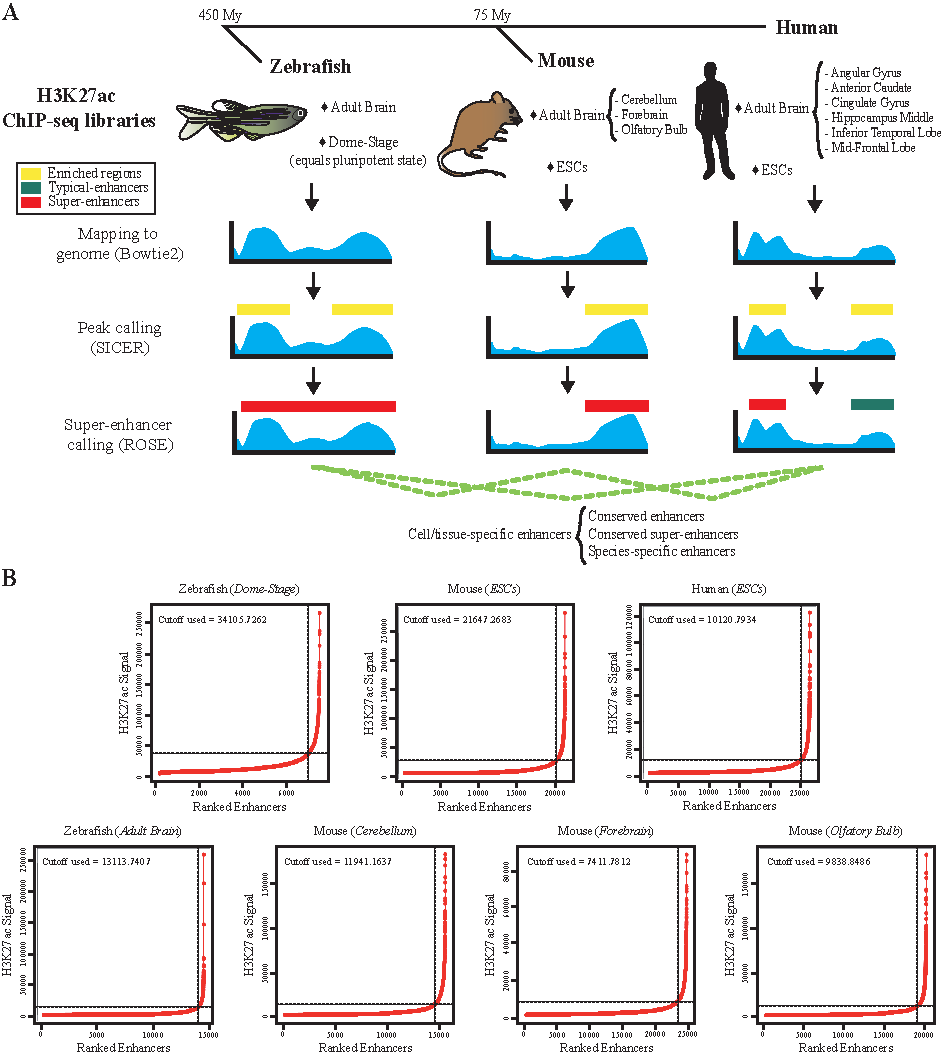
\includegraphics[width=16cm,height=18cm]{./figures/Figure_1.pdf}
  			\caption[Identification]{\textbf{Identification of enhancers in vertebrate genomes.} (A) H3K27ac ChIP-seq data sets analyzed and pipeline applied for the identification of typical-enhancers and super-enhancers. Evolutionary distances between the three organism are depicted in the upper dendrogram in million years (My). (B) Saturation curves of H3K27ac density across enhancers for the data sets analyzed in this study. The x-axis shows the number of ranked enhancers by density identified in each data set and their corresponding densities are plotted in the y-axis. Horizontal dot lines represent density cutoffs used for the identification of super-enhancers, and vertical dot lines demark super-enhancers from typical-enhancers.}
			\label{Identification}
			\rule{\textwidth}{0.25mm}
		\end{figure}

		The existence of long clusters of stretch enhancers in mammalian cells and tissues has previously been reported (Whyte et al., 2013; Lov\'en et al., 2013; Hnisz et al., 2013). These clusters of hyperactive chromatin or super-enhancers were originally identified based on ChIP-seq data that marked the genomic positions of master transcription factors in embryonic stem cells (ESCs) and Mediator sub-units (Whyte et al. 2013). However, it has been reported that the ChIP-seq data of additional transcriptional coactivators and histone marks might also contribute to the identification and refinement of super-enhancer locations. Specifically, the H3K27ac has been deamed as a robust epigenetic mark for predicting super-enhancers (Hnisz et al. 2013). Thus, to assess whether stretch enhancers are present outside of mammals and to create vertebrate maps of conventional enhancers further referred to as "typical-enhancers" and stretch enhancers further referred to as "super-enhancers", we based our predictions uniquely on zebrafish, mouse and human H3K27ac ChIP-seq data. For our analyses, we focused on the complex tissue of adult brain as well as ESC lines. We considered the early embryonic dome-stage of zebrafish as equivalent to the pluripotent state of mouse and human ESCs (Schier and Talbot, 2005; Vastenhouw et al., 2010).\\

		\begin{figure}[!h]
			\centering
			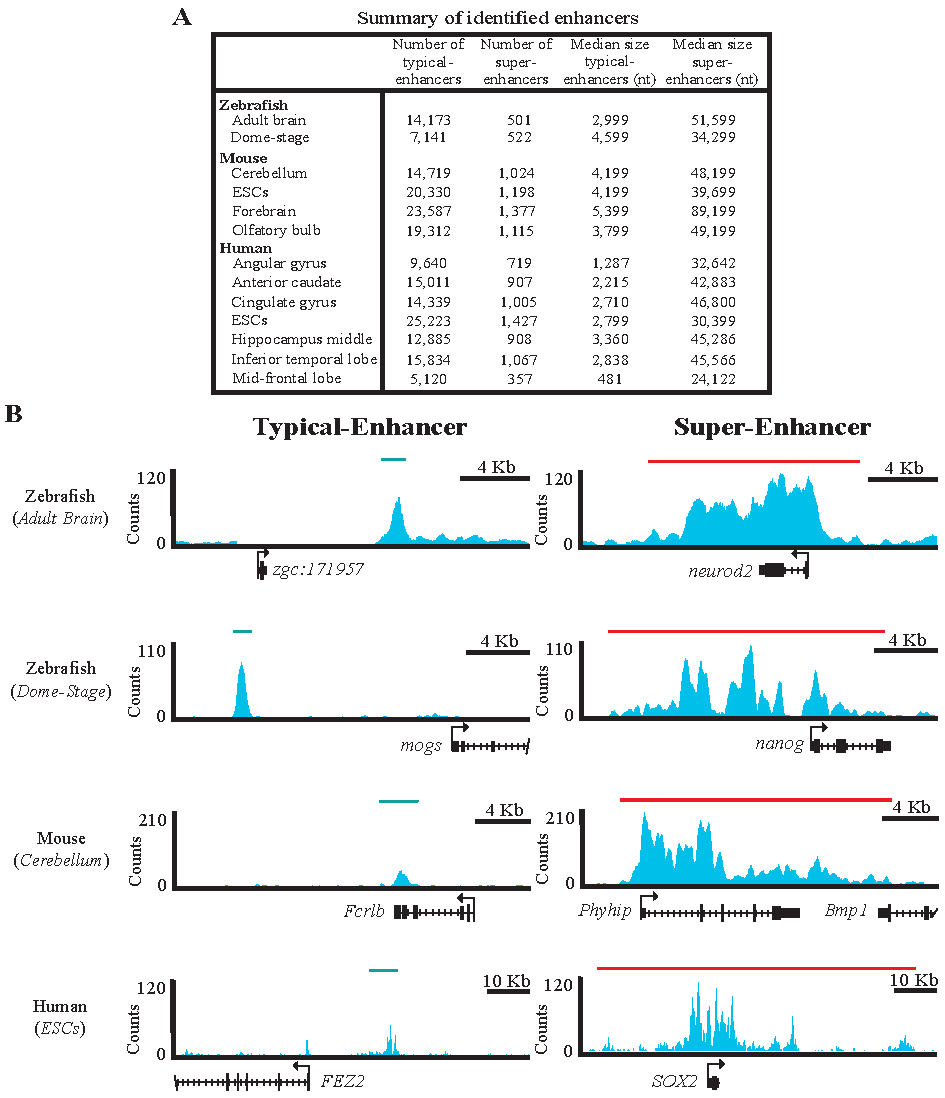
\includegraphics[width=16cm,height=18.6cm]{./figures/Figure_2.pdf}
  			\caption[Super-enhancers]{\textbf{Comparisons of typical-enhancers and super-enhancers.} (A) Summary table with the numbers of identified enhancers and their median sizes. (B) Genome tracks displaying examples of typical-enhancers and super-enhancers in the same data set for zebrafish, mouse and human. H3K27ac ChIP-seq profiles are shown in tag counts. Green and red bars over profiles represent typical-enhancers and super-enhancers respectively. Gene models are drawn below the binding profiles.}
			\label{Super-enhancers}
			\rule{\textwidth}{0.25mm}
		\end{figure}

		We took advantage of the available H3K27ac ChIP-seq data sets (Rada-Iglesias et al., 2011; Mouse ENCODE Consortium, 2012; Bogdanovic et al., 2012; Chadwick, 2012; Nord et al., 2013) and subjected them to a modified enhancer/super-enhancer computational identification pipeline following the same strategy used by Hnisz et al. (2013). Enhancer maps for the human adult brain data sets were already available (Hnisz et al., 2013), therefore, we used those published maps for all the analyses. Given that no zebrafish brain ChIP-seq data has been published, we generated H3K27ac ChIP profiles by sequencing two biological replicates prepared from whole adult brains of mixed genders. The included data sets and the pipeline applied for identification of typical-enhancers and super-enhancers are described in Figure 1A. First, we re-analyzed all available H3K27ac ChIP data sets by mapping the libraries to their corresponding reference genomes. Reads with low mapping quality were discarded from our further analyses. \texttt{SICER} was used to reveal genomic regions with H3K27ac enrichment (Zang et al., 2009), which represents regions of constitutive enhancers. Next, to classify constitutive enhancers as typical-enhancers or super-enhancers, we implemented the \texttt{ROSE} program (Whyte et al., 2013; Lov\'en et al., 2013). Briefly, \texttt{ROSE} stitches together neighboring constitutive enhancers using a maximal distance of 12.5 Kb creating long unique regions. After stitching, ChIP-seq densities are calculated for all regions and plotted by increasing density. To calculate the cutoff density to distinguish super-enhancers from typical-enhancers, the density value on the curve with a tangent equal to 1 is determined. This value represents the point at which the H3K27ac density starts to rapidly increase. All of the regions with a density higher than this value are considered as super-enhancers, while the remaining are classified as typical-enhancers (Figure 1B).\\

		Following this approach, We successfully identified super-enhancers in mouse, human and non-mammalian zebrafish data sets, and we found that zebrafish super-enhancers share key features with published mammalian super-enhancers such as their abundance and size (Figure 2A). For example, more enhancers were classified as typical-enhancer than as super-enhancer in all data sets and the median lengths of super-enhancers were longer than those of typical-enhancers. In general, super-enhancers spanned tens of thousands of base pairs, while typical-enhancers spanned only a few thousand base pairs (Figure 2B). It should be noted that with our approach we identified more super-enhancers for mouse ESCs than was originally reported (Whyte et al., 2013), 1198 versus 231, respectively. One possibility for this difference is that Whyte et al. first identified constitutive enhancers based on ChIP-seq data for Oct4, Sox2 and Nanog and then ranked them by Mediator signal, to refine their predictions. Nevertheless, based only on H3K27ac data we identified \(\sim79\)\% of the published super-enhancers, implying that by using uniquely this epigenetic mark and following our pipeline, it is possible to distinguish true super-enhancers from typical-enhancers.\\

	\subsection{Comparison of enhancer and super-enhancer attributes across vertebrates}

		To further assess if the main attributes characterizing mammalian typical-enhancers and super-enhancers were conserved across vertebrates, we first created metagene representations for all of the libraries analyzed (Figure 3A). These representations show the average H3K27ac density along typical-enhancers and super-enhancers in relation to their length. It is noticeable that for all data sets, the median size of typical-enhancers and super-enhancers differs by orders of magnitude and that super-enhancers accumulate most of the H3K27ac signal. Next, we investigated the correlation between H3K27ac density and length for the classification of super-enhancers. Although the correlation increased proportionally and the longest regions have higher densities, in some of the data sets there were long regions spanning up to 150 Kb with low H3K27ac density and subsequently were classified as typical-enhancers (Figure 3B).\\

		\begin{figure}[!h]
			\centering
			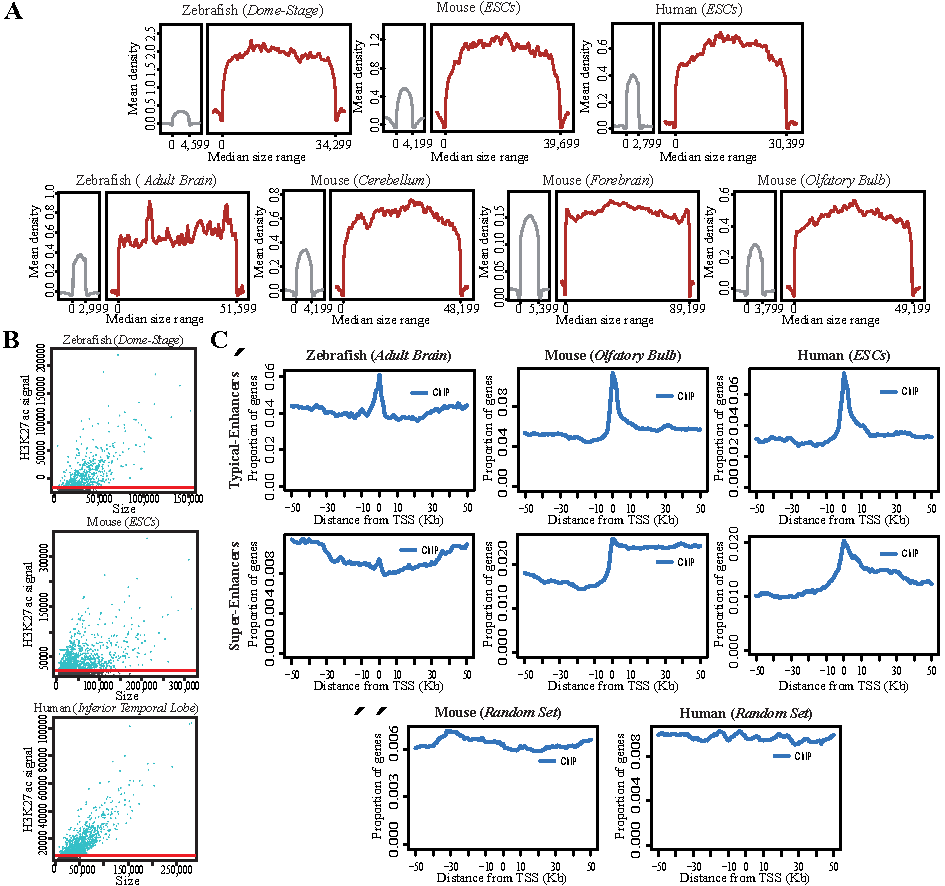
\includegraphics[width=16cm,height=15cm]{./figures/Figure_3.pdf}
  			\caption[Features]{\textbf{Representative features of vertebrate super-enhancers.} (A) Metagene representations of normalized H3K27ac density for typical-enhancers (grey curve) and super-enhancers (red curve). The y-axis shows the average H3K27ac density across enhancers. The regions displayed in the x-axis illustrate typical-enhancers and super-enhancers flanked by 3 Kb of adjacent sequence. Enhancer starts and ends are scaled relatively to median lengths. (B) Relationship between H3K27ac density (y-axis) and enhancer size (x-axis). Blue dots represent super-enhancers and the red line indicates the density cutoff used for the classification of enhancers. (C) Density plots with the proportion of genes for which the indicated locations around the TSS (x-axis) are covered by a typical-enhancer or a super-enhancer in the analyzed data sets (') and in randomly generated regions ('').}
			\label{Features}
			\rule{\textwidth}{0.25mm}
		\end{figure}

		It has also been noted that super-enhancers tend to overlap with the genes with which they are associated (Whyte et al., 2013; Lov\'en et al., 2013; Hnisz et al., 2013). Thus, we decided to examine if this tendency was maintained in our analyzed data sets. We observed that contrary to typical-enhancers, which cover the nearest regions surrounding the TSS, mouse and human super-enhancers tend to be more present in the down-stream region of the TSS. However, the distributions for zebrafish super-enhancers did not show the same tendency (Figure 3C). And given that only in 39 cases the distance between two super-enhancers was shorter than 100 Kb and the average distance was 2.2 Mb, the observed distribution could not be explained by problems with the stitching of adjacent super-enhancers around TSSs. Therefore, the distribution suggests that the relationship between super-enhancers and their target genes in zebrafish is different from that in mammals. Another explanation for this difference could be that it is a consequence of the incomplete gene annotation in zebrafish compared to that of mouse and human genomes. To eliminate the possibility that mouse and human super-enhancers were overlapping genes merely because of their long sizes, a random set of regions was analyzed for each genome. These random regions were not preferentially associated with a particular region within the 100 Kb window analyzed (Figure 3C).\\

	\subsection{Super-enhancers associate with cell-type specific genes}

		We annotated genes to typical-enhancers and super-enhancers following a strategy based on genomic proximity. Upon Gene Ontology (GO) enrichment analysis, we found that most of the annotated genes were related to development, neural processes and ESCs maintenance. As it has been reported by Whyte et al. (2013), Lov\'en et al. (2013) and Hnisz et al. (2013), the annotations for super-enhancers included key identity genes such as \textit{sox2}, \textit{nanog}, \textit{klf4}, \textit{wnt11}, \textit{prdm14}, \textit{foxh1}, and \textit{ptch2} (Heisenberg et al., 2000; Takahashi and Yamanaka, 2006; Burton et al., 2013; Holtz et al., 2013; Takahashi et al., 2014) in the ESCs data sets. By contrast, in the brain data sets we found identity genes involved in neural development, synaptic communication and neural stem quiescence such as \textit{neurod2}, \textit{neurexin1}, \textit{nfix}, \textit{zic1} and \textit{zic4} (Rissone et al., 2007; Eisen et al., 2008; Sato and Takeda, 2013; Martynoga et al., 2013). Interestingly, the three genes coding for the master transcription factors in ESCs were only associated with super-enhancers in the mouse ESCs data set, while in the zebrafish data set only \textit{nanog} was associated with a super-enhancer and the other two genes were associated with typical-enhancers. We found that in the human ESCs, only \textit{SOX2} and \textit{NANOG} had super-enhancers associated with them and, strikingly, the 6 Mb region surrounding \textit{OCT4} was depleted of H3K27ac signal, a result that we reproduced using another two independent human ESCs data sets (Chadwick, 2012; Loh et al., 2014; data not shown).\\

		To investigate whether the key identity genes that we identified were uniquely associated to a super-enhancer in adult brain or ESCs but not in the other cell/tissue type, we focused on three examples of key identity genes with a conserved super-enhancer in zebrafish, mouse and human. We selected the forkhead transcription factor \textit{foxh1} for ESCs and the couple \textit{zic1} and \textit{zic4} for adult brain data sets. It has been reported that FOXH1 is able to enhance the efficiency of reprogramming of human differentiated cells to generate induced pluripotent stem cells (Takahashi et al., 2014). Although no super-enhancers were associated to this gene in the brain, we found that in ESCs of all three organisms, the super-enhancer was present and overlapped the entire gene body of \textit{foxh1}. Only in mouse cerebellum, two typical-enhancers were found in the neighboring area (Figure 4A). On the other hand, expression of \textit{zic1} and \textit{zic4} is required for the normal morphogenesis of the hindbrain ventricle controlled by proliferation and fate specification in zebrafish (Eisen et al., 2008). Our data showed that, similar to \textit{foxh1}, brain super-enhancers covered the entire gene body of both \textit{zic1} and \textit{zic4}  and spanned through the up-stream and down-stream regions. By contrast, in zebrafish, mouse and human ESCs these genes were associated with typical-enhancers, suggesting that \textit{zic1} and \textit{zic4} might also be expressed in ESCs but its expression might not be as essential as in the brain (Figure 4B).\\

		\begin{figure}[!h]
			\centering
			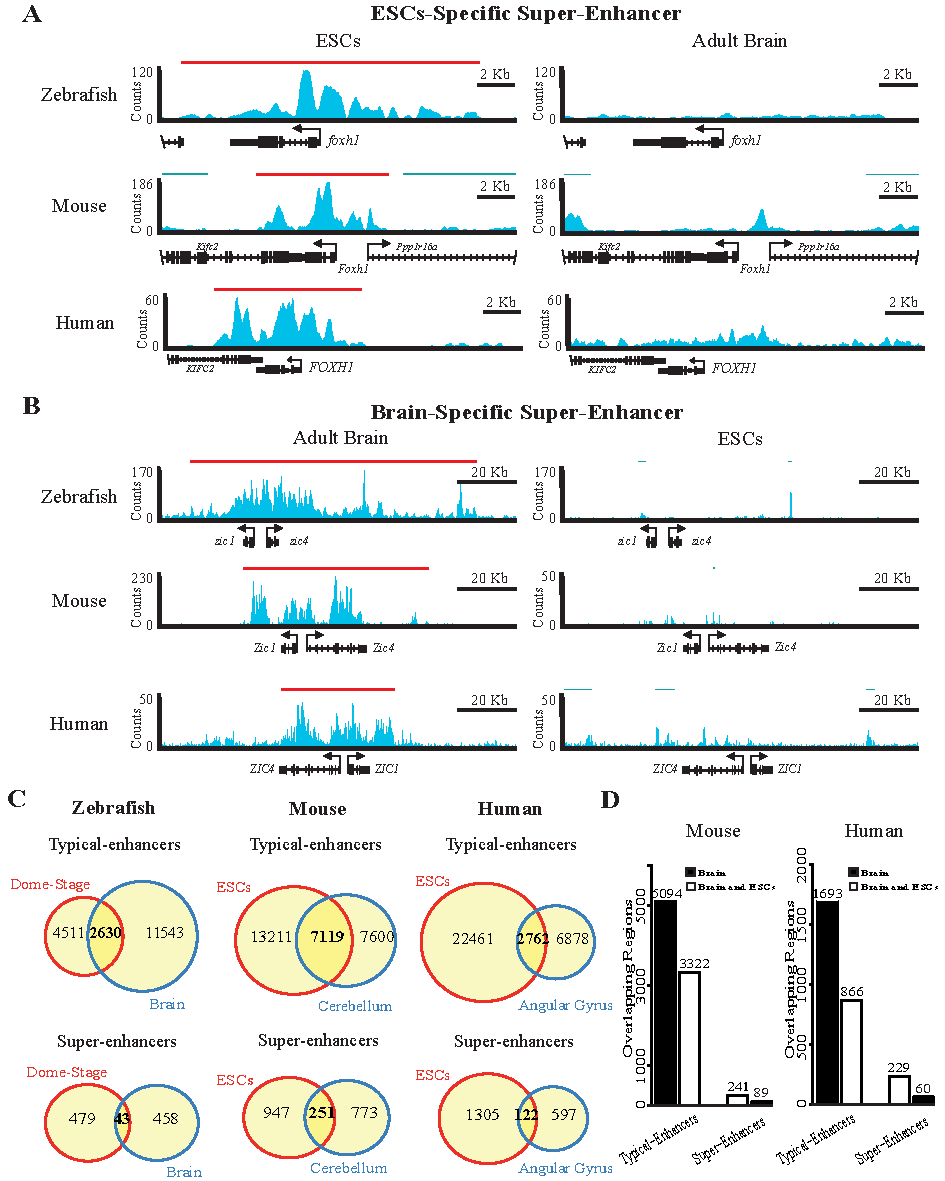
\includegraphics[width=15cm,height=17cm]{./figures/Figure_4.pdf}
  			\caption[Specificity]{\textbf{Significant fractions of enhancers and super-enhancers are cell/tissue-specific.} (A) Examples of identity genes associated with a super-enhancer across vertebrates. Genome tracks are displayed as described in Figure 2B. (B) Venn diagrams with the global overlaps of typical-enhancers and super-enhancers in the different data sets. (C) Barplots representing the number of enhancer overlapping regions among brain data sets (black bar) or among brain and ESCs data sets (white bar) for mouse and human.}
			\label{Specificity}
			\rule{\textwidth}{0.25mm}
		\end{figure}

		Next, we globally compared typical-enhancers and super-enhancers between adult brain and ESCs. To obtain the sets of overlapping regions in the genomes, we compared the maps of typical-enhancers and super-enhancers between data sets from the same organism. We observed that for zebrafish, mouse and human, the number of overlapping regions is higher for typical-enhancers than for super-enhancers (Figure 4C). This observation is consistent with the idea that super-enhancers are generally associated with cell-type specific genes and thus, we would expect that only a small subset of super-enhancers are shared between different cell types. Specifically, we expected that some genes coding for transcriptional cofactors such as Mediator would be associated with super-enhancers in different cell-types. Given that for mouse and human, data sets for different brain regions are available, we performed multiple comparisons of the typical-enhancer and super-enhancer maps to obtain a global panorama of brain enhancers compared with ESCs enhancers. As seen in the pairwise comparisons, the number of overlapping regions among the typical-enhancers was higher than for super-enhancers in mouse and human. It also should be noted that, in general, the number of overlapping regions between different brain data sets is higher than for overlapping regions between brain and ESC data sets (Figure 4D). This data supports the idea that the enhancer landscape changes according to cell types and that the subset of enhancers and super-enhancers identified and analyzed is highly specific to that particular cell type or tissue.\\

	\subsection{Conservation of enhancers and super-enhancers in vertebrate genomes}

		\begin{figure}[!h]
			\centering
			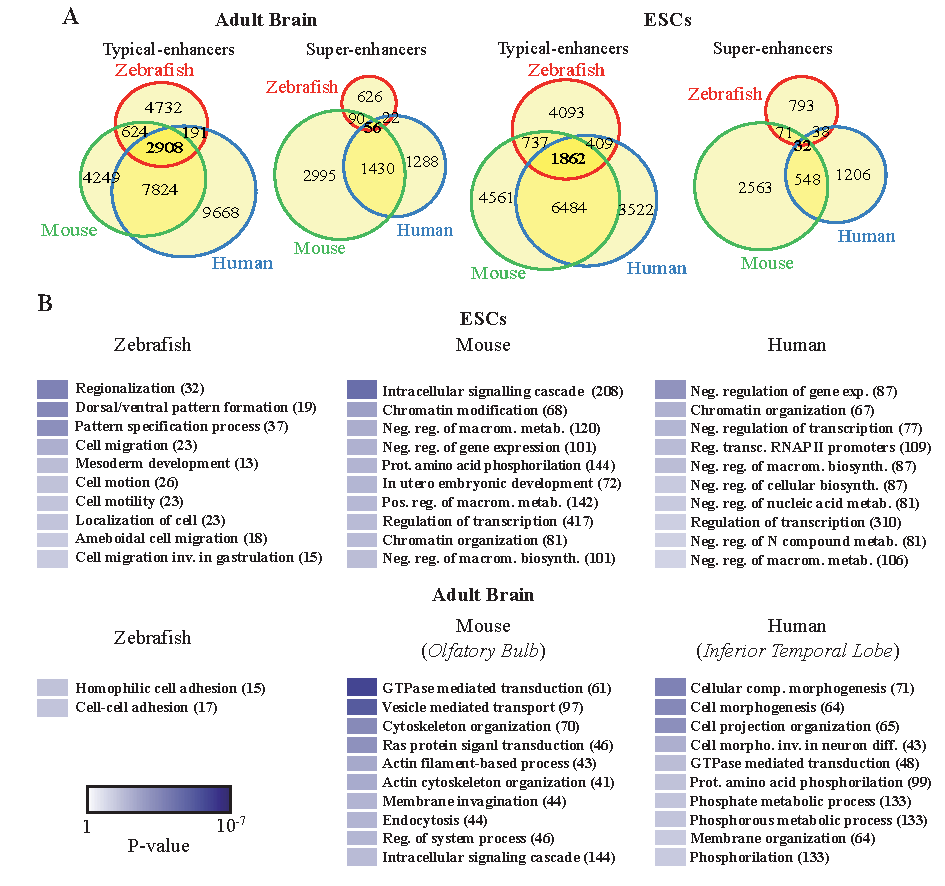
\includegraphics[width=16cm,height=16cm]{./figures/Figure_5.pdf}
  			\caption[Conservation]{\textbf{Conservation of enhancer and super-enhancer target genes and functions across vertebrate genomes.} (A) Venn diagrams displaying the overlaps of enhancer maps for zebrafish, mouse and human. (B) Top ten molecular function GO terms enriched for genes associated with super-enhancers. Adjusted p-values for the GO terms are displayed in a color scale. Only terms with adjusted p-values $<0.06$ are considered as significantly enriched.}
			\label{Conservation}
			\rule{\textwidth}{0.25mm}
		\end{figure}

		Taking into account that super-enhancers are associated with genes that specify cell identity and also the fact that most of these key regulator genes are conserved across organisms, we next investigated if typical-enhancers and super-enhancers were associated with the same genes across vertebrates. We performed inter-species comparisons based on gene name and found that, among enhancer maps, both typical-enhancers and super-enhancers for the same genes were conserved. For the adult brain and ESCs comparisons, more genes associated with typical-enhancers (2908 for adult brain and 1862 for ESCs) than with super-enhancers (56 for adult brain and 32 for ESCs) were shared between zebrafish, mouse and human. The conservation of enhancer-associated target genes was higher between mouse and human than when they were compared to zebrafish (Figure 5A), consistent with the evolutionary distance among these species. The lists of common genes associated with a super-enhancer included those related to cell fate identity such as \textit{nfix}, \textit{foxh1}, \textit{neurod2} and \textit{sox2}. In addition, genes that code for transcriptional coactivators were also present among these lists, which is logical considering that super-enhancers are highly occupied by transcriptional cofactors. High levels of these proteins are required in the cell, and it has been reported that super-enhancers can trigger higher rates of transcription than typical-enhancers (Whyte et al., 2013), which could explain the association of super-enhancers to those genes. It should be noted that the comparisons were performed only based on the gene name. Thus, the observed overlaps are likely an underestimation of the real conservation because ortholog genes do not always share the same gene name.\\

		An alternative strategy to determine the conservation of super-enhancers is to analyze if the biological processes with which their associated genes are involved, remain similar in zebrafish, mouse and human. We performed GO enrichment analysis and found that ESCs data sets were mainly enriched for terms relative to transcription regulation, while for the dome-stage data set the top terms were related to patterning and cell migration. For the adult brain data sets, among the top terms cytoskeleton organization, morphogenesis and cell-adhesion (Figure 5B). Although the terms found for the zebrafish brain data set were similar to those found for the mouse and human data sets, only two of the terms had significant adjusted p-values. Most likely, this is a consequence of the zebrafish background that is considered by the program used for the enrichment of GO terms, as only a reduced number of terms got significant p-values also for the dome-stage data set. For all data sets in zebrafish, mouse and human, we found that transcription regulator activity was among the top molecular function terms. These results highlight the frequent associations that exist between super-enhancers and regulators of transcription.\\



	\section{Conclusions and Outlook}

	Increasing evidence suggests that super-enhancers drive cell fate through regulation of key identity genes (Whyte et al., 2013; Lov\'en et al., 2013; Parker et al., 2013; Hnisz et al., 2013; Siersb\ae k et al., 2014). However, there is a lack of mechanistic data for super-enhancers, and it remains to be elucidated if they are a cause or a consequence of the high levels of transcription measured for their target genes. Therefore, the establishment of animal models, such as zebrafish, for the \textit{in vivo} analysis of super-enhancers is paramount to develop functional analyses that could address these questions. Here, we have focused on the generation of enhancer maps for adult brain and dome-stage zebrafish embryos to assess if super-enhancers are present in non-mamalian cells and tissue. We successfully identified super-enhancers in zebrafish data sets and observed that the number of super-enhancers is proportional to that obtained for mouse and human data sets, after normalizing for genome size. Importantly, we also extended the list of known of enhancers for both mouse and human.\\

	One aspect that has not been taken into account for the refinement of typical-enhancers and super-enhancers maps is that the H3K27ac mark is found in both enhancers and promoters (Rada-Iglesias et al., 2011) and, thus, does not directly distinguish between these two types of regions. As a consequence, it is necessary to apply an additional filter to distinguish between these two types of regions. One possible filter would be to establish exclusion zones near TSSs. Another possibility would be to obtain profiles for trimethylation in histone H3 at lysine 4 (H3K4me3), which is enriched in promoters, and compare these profiles to H3K27ac profiles.\\

	We observed that, in general, zebrafish typical-enhancers and super-enhancers shared key features with their counterparts in mouse and human, except for the enrichment distribution around TSSs. Because we only analyzed two zebrafish data sets it would be interesting to extend the analysis to more libraries to see if the obtained distributions for super-enhancers could be reproduced.\\

	In agreement with the previous analyses of mouse and human data sets, zebrafish enhancers were highly cell/tissue specific. We found that the overlap between typical-enhancers in different data sets was higher than that observed for super-enhancers. An aspect that remains to be determined is whether the overlap observed for super-enhancers is significant or whether it is comparable to the overlap that we could be obtained for random regions.\\

	Our analysis showed that a fraction of putative gene targets of typical-enhancers and super-enhancers is conserved in vertebrate genomes, and, as expected, this conservation is higher between mouse and human than when compared to zebrafish. Moreover, the biological processes, in which super-enhancer target genes are involved, are conserved in the equivalent cells/tissues across vertebrates. However, to obtain better estimations of enhancer conservation, we should consider additional approaches. For example, comparisons based on sequence rather than gene name could overcome the differences in gene nomenclature among the three organisms. It would also be interesting to evaluate the relationship between transcription factors and super-enhancers and to analyze if transcription factor hotspots are also conserved among vertebrates.\\



	\section*{Acknowledgements}

		I would like to thank my family and friends for all their support and encouragement during the last months. I would especially like to thank \textit{"Los Morros"} for sharing wonderful adventures with me in Paris. Moreover, I am very grateful to Alena Shkumatava for giving me the opportunity to perform my internship in her inspiring team at the Institut Curie. I would also like to thank members of the Shkumatava lab for helpful discussions, and especially Allison Mallory for comments on the manuscript. Finally, I would like to thank Valentina Boeva and Emmanuel Barillot for their supervision in the development of this project.\\

	\begin{thebibliography}{40}
	\bibitem[]{Paused-pol} Adelman, K., Lis, J. T. 2012. Promoter-proximal pausing of RNA polymerase II: emerging roles in metazoans. \emph{Nat Rev Genet} \textbf{13:} 720--731.
	\bibitem[]{zf-dataset} Bogdanovic, O., et al. 2012. Dynamics of enhancers chromatin signatures mark the transition from pluripotency to cell specification during embryogenesis. \emph{Genome Res} \textbf{22:} 2043--2053.
	\bibitem[]{nebula} Boeva, V., Lermine, A., Barette, C., Guillouf, C., Barillot, E. 2012. Nebula--a web-server for advanced ChIP-seq data analysis. \emph{Bioinformatics} \textbf{28:} 2517--2519.
	\bibitem[]{prdm14} Burton, A., et al. 2013. Single-cell profilling of epigenetic modifiers identifies PRDM14 as an inducer of cell fate in the mammalian embryo. \emph{Cell Rep} \textbf{5:} 687--701.
	\bibitem[]{roadmap} Chadwick, L. H. 2012. The NIH Roadmap Epigenomics Program data source. \emph{Epigenomics} \textbf{4:} 317--324.
	\bibitem[]{disease} Creyghton, M. P., et al. 2010. Histone H3K27ac separates active from poised enhancers and predicts developmental state. \emph{Proc Natl Acad Sci} \textbf{107:} 21931--21936.
	\bibitem[]{Darnell} Darnell, J. 2011. RNA: Life's Indispensable Molecule. \emph{Cold Spring Harbor Laboratory Press} \textbf{ISBN: 978-1-936113-19-4}.
	\bibitem[]{david} Dennis, G. Jr., et al. 2003. DAVID: Database for Annotation, Visualization, and Integrated Discovery. \emph{Genome Biology} \textbf{4:} P3.
	\bibitem[]{zic1} Eisen, G. E., Choi, L. Y., Millen, K. J., Grinblat, Y., Prince, V. E. 2008. Zic1 and Zic4 regulate zebrafish roof plate specification and hindbrain ventricle morphogenesis. \emph{Dev Biol} \textbf{314:} 376--392.
	\bibitem[]{findpeaks} Fejes, A. P., et al. 2008. FindPeaks 3.1: a tool for identifying areas of enrichmentfrom massively parallel short-read sequencing technology. \emph{Bioinformatics} \textbf{24:} 1729--1730.
	\bibitem[]{wnt11} Heisenberg, C. P., et al. 2000. Silberblick/Wnt11 mediates convergent extension movements during zebrafish gastrulation. \emph{Nature} \textbf{405:} 76--81.
	\bibitem[]{Super-enhancers3} Hnisz, D., et al. 2013. Super-enhancers in the control of cell identity and disease. \emph{Cell} \textbf{155:} 934--947.
	\bibitem[]{ptch2} Holtz, A. M., et al. 2013. Essential role for ligand-dependent feedback antagonism of vertebrate hedgehog signaling by PTCH1, PTCH2 and HHIP1 during neural patterning. \emph{Development} \textbf{140:} 3423--3434.
	\bibitem[]{zf-genome} Howe, K., et al. 2013. The zebrafish reference genome sequence and its relationship to the human genome. \emph{Nature} \textbf{496:} 498--503.
	\bibitem[]{interactome} Kieffer-Kwon, K., et al. 2013. Interactome maps of mouse gene regulatory domains reveal basic principles of transcriptional regulation. \emph{Cell} \textbf{155:} 1507--1520.
	\bibitem[]{TIF} Koch, F., et al. 2011. Transcription initiation platforms and GTF recruitment at tissue-specific enhancers and promoters. \emph{Nat Struct Mol Biol} \textbf{18:} 956--963.
	\bibitem[]{bowtie2} Langmead B., Salzberg S. L. 2012. Fast gapped-read alignment with Bowtie 2. \emph{Nature Methods} \textbf{9:} 357--359.
	\bibitem[]{samtools} Li H., et al. 2009. The Sequence alignment/map (SAM) format and SAMtools. \emph{Bioinformatics} \textbf{25:} 2078--2079.
	\bibitem[]{H7} Loh, K. M., et al. 2014. Efficient endoderm induction from human pluripotent stem cells by logically directing signals controlling lineage bifurcations. \emph{Cell Stem Cell} \textbf{14:} 237--252.
	\bibitem[]{Super-enhancers2} Lov\'en, J., et al. 2013. Selective inhibition of tumor oncogenes by disruption of super-enhancers. \emph{Cell} \textbf{153:} 320--334.
	\bibitem[]{nfix} Martynoga, B., et al. 2013. Epigenomic enhancer annotation reveals a key role of NFIX in neural stem cell quiescence. \emph{Genes Dev} \textbf{27:} 1769--1786.
	\bibitem[]{encode} Mouse ENCODE Consortium. 2012. An encyclopedia of mouse DNA elements (Mouse ENCODE). \emph{Genome Biology} \textbf{13:} 418.
	\bibitem[]{mouse_develop} Nord, A. S., et al. 2013. Rapid and pervasive changes in genome-wide enhancer usage during mammalian development. \emph{Cell} \textbf{155:} 1521--1531.
	\bibitem[]{stretch-enhancers} Parker, S. C. J., et al. 2013. Chromatin stretch enhancer states drive cell-specific gene regulation and harbor human disease risk variants. \emph{Proc Natl Acad Sci} \textbf{29:} 17921--17926.
	\bibitem[]{bedtools} Qunian, A. R., Hall, I. M. 2013. BEDTools: a flexible suite of utilities for comparing genomic features. \emph{Bioinformatics} \textbf{26:} 841--842.
	\bibitem[]{neurexin} Rissone, A., et al. 2007. Comparative genome analysis of the neurexin gene family in Danio rerio: Insights into their functions and evolution. \emph{Mol Biol Evol} \textbf{24:} 236--252.
	\bibitem[]{H3K27ac-2} Rada-Iglesias, A., et al. 2011. A unique chromatin signature uncovers early developmental enhancers in humans. \emph{Nature} \textbf{470:} 279--283.
	\bibitem[]{neurod} Sato, A., Takeda, H. 2013. Neuronal subtypes are specified by the level of neurod expression in the zebrafish lateral line. \emph{J Neurosci} \textbf{33:} 556--562.
	\bibitem[]{dome1} Schier, A. F., Talbot, W. S. 2005. Molecular genetics of axis formation in zebrafish. \emph{Annu Rev Genet} \textbf{39:} 561--613.
	\bibitem[]{Review2} Shlyueva, D., Stampfel, G., Stark, A. 2014. Transcriptional enhancers: from properties to genome-wide predictions. \emph{Nat Rev Genet} \textbf{15:} 272--286.
	\bibitem[]{first-hotspots} Siersb\ae k, R., et al. 2011. Extensive chromatin remodelling and establishment of transcription factor 'hotspots' during early adipogenesis. \emph{EMBO} \textbf{30:} 1459--1472.
	\bibitem[]{hotspots} Siersb\ae k, R., et al. 2014. Transcription factor cooperativity in early adipogenic hotspots and super-enhancers. \emph{Cell Rep} \textbf{7:} 1--13.
	\bibitem[]{hotspots-architecture} Siersb\ae k, R., et al. 2014. Molecular architecture of transcription factor hotspots in early adipogenesis. \emph{Cell Rep} \textbf{7:} 1--9.
	\bibitem[]{Review1} Smith, E., Shilatifard, A. 2014. Enhancer biology and enhanceropathies. \emph{Nat Struct Mol Biol} \textbf{21:} 210--219.
	\bibitem[]{foxh1} Takahashi, K., et al. 2014. Induction of pluripotency in human somatic cells via a transient state resembling primitive streak-like mesendoderm. \emph{Nat Commun} \textbf{5:} 3678.
	\bibitem[]{sox2-klf4} Takahashi, K., Yamanaka, S. 2006. Induction of pluripotent stem cells from mouse embryonic and adult fibroblast cultures by defined factors. \emph{Cell} \textbf{126:} 663--676.
	\bibitem[]{igv} Thorvaldsd\'ottir, H., Robinson, J. T., Mesirov, J. P. 2012. Integrative Genomics Viewer (IGV): high-performance genomics data visualization and exploration. \emph{Brief Bioinform} \textbf{14:} 178--192.
	\bibitem[]{dome2} Vastenhouw, N. L., et al. 2010. Chromatin signature of embryonic pluripotency is established during genome activation. \emph{Nature} \textbf{464:} 922--926.
	\bibitem[]{Super-enhancers1} Whyte, W. A., et al. 2013. Master transcription factors and mediator establish super-enhancers at key cell identity genes. \emph{Cell} \textbf{153:} 307--319.
	\bibitem[]{sicer} Zang, C., et al. 2009. A clustering approach for identification of enriched domains from histone modification ChIP-Seq data. \emph{Bioinformatics} \textbf{25:} 1952--1958.
\end{thebibliography}



\end{document}

